\documentclass[compress,xcolor=table,hyperref]{beamer}
\usepackage{ctex}
% Packages
\usepackage[english]{babel}
\usepackage[utf8]{inputenc}
\usepackage[T1]{fontenc}
\usepackage{datetime}
\usepackage{multicol}
\setbeamertemplate{bibliography item}[text]
\usepackage{multirow}
\usepackage{hyperref}
% Possible options of the package (add/remove below in \usetheme call):
%  - nosectionpages: no pages between sections
%  - flama: use flama font, requires xelatex/lualatex + the font to compile
%  - compressminiframes: put the heading list bullets indications pages on 1 line
\usetheme[compressminiframes]{sorbonne}
\usepackage{ragged2e}
% Title page
\title{\vspace{1em}FRAUD DETECTION \newline Based On GAT and DRSA}
%\foottitle{Lorem Ipsum Dolor Sit Amet} % optional, printed at the bottom of the slides, by default same as title, can be useful to rewrite when title has a newline for example
\subtitle{} % optional subtitle
\date{\vspace{3em}\formatdate{23}{04}{2020}}
\author{FuXinlan XingYuyan ZhuChaona}
% \institute{LIP6 - Sorbonne Université} % Optional

% Biblatex
\usepackage[backend=bibtex, style=authoryear, citestyle=authoryear]{biblatex}
\bibliography{library.bib}
\renewcommand*{\bibfont}{\footnotesize}


%%%%
%% BEGIN OF SLIDES
%%%%

\begin{document}

\begin{frame}[plain]
	\titlepage
	\setcounter{framenumber}{0}
\end{frame}


\section{Introduction and Research Status
	of Fraud Detection} 

\begin{frame}{Problem introduction}
	
	\begin{block}{Difficulties in fraud detection:}
		\vspace{-1em}
		\begin{multicols}{2}
			\begin{itemize}
			\item
			Difficult problem definition                 
			\item high labeling cost
			\item	few black samples              
			\item          white samples are noisy;
			\item	fraudsters are evolving
		\end{itemize}
		\end{multicols}
	\end{block}
\begin{center}
		\begin{minipage}{0.45\linewidth}
		\begin{figure}[h]
			\centering
			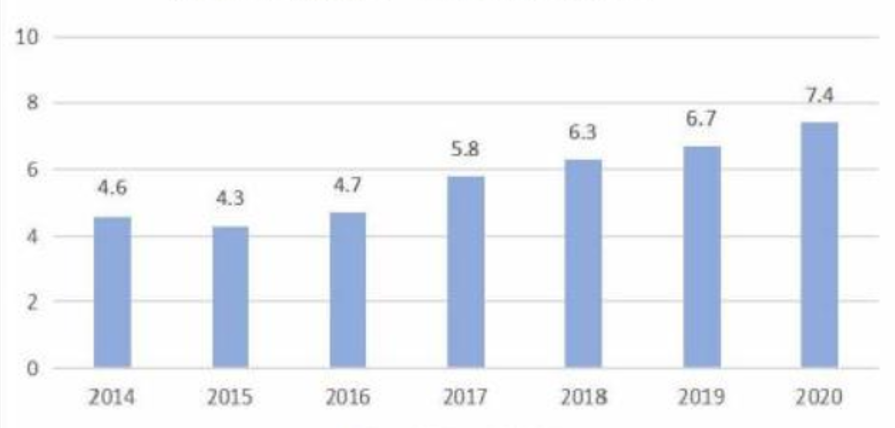
\includegraphics[width=1.1\linewidth]{images/fig1}
			\caption{Number of credit cards (100 million)}
			\label{fig:fig1}
		\end{figure}
	\end{minipage}
	\hspace{0.07\linewidth}
	\begin{minipage}{0.45\linewidth}
		\begin{figure}[h]
			\centering
			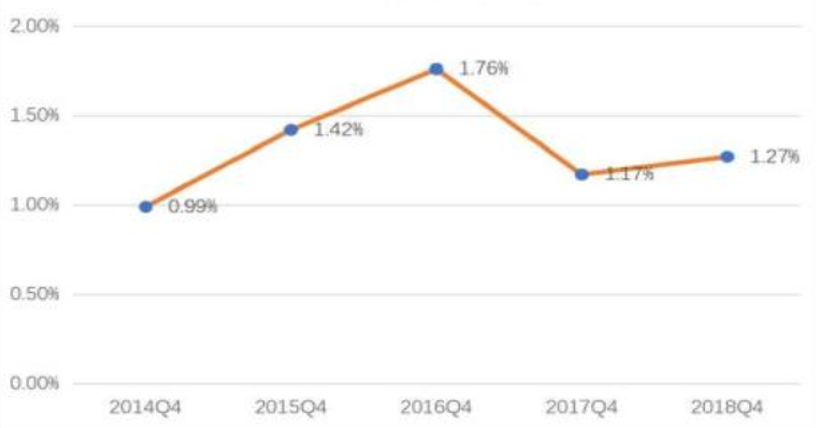
\includegraphics[width=0.9\linewidth]{images/fig2}
			\caption{Credit card loss rate}
			\label{fig:fig1}
		\end{figure}
	\end{minipage}
\end{center}
\end{frame}
\begin{frame}{Literature review}
\begin{table}[h]
	\centering
	\renewcommand\arraystretch{1.2}
\scalebox{0.75}[0.75]{\begin{tabular}{|c|l|l|l|l|l|}
		\hline
		\multirow{2}{*}{} & \multicolumn{2}{c|}{Supervised learning} & \multicolumn{1}{c|}{unsupervised learning} & \multicolumn{2}{c|}{semi-supervised learning} \\ \cline{2-6} 
		& \multicolumn{2}{c|}{Ref{[1,2]}}           & \multicolumn{1}{c|}{Ref{[3]}}             & \multicolumn{2}{c|}{Ref{[4,5]}}                \\ \hline
		Advantage &
		\multicolumn{2}{l|}{\begin{tabular}[c]{@{}l@{}}The recall rate can\\ reachthe limit of\\ the quality of the\\ existing data samples\\ (Fully adjust the\\ parameters)\end{tabular}} &
		\begin{tabular}[c]{@{}l@{}}Can discover\\ new anomalies\end{tabular} &
		\multicolumn{2}{l|}{\begin{tabular}[c]{@{}l@{}}The recall rate is\\ very good,the unknown\\ maliciousness can be\\ found, the resistance\\ is good, and the\\ timeliness is also\\ better than supervised\\ learning\end{tabular}} \\ \hline
		Disadvantage &
		\multicolumn{2}{l|}{\begin{tabular}[c]{@{}l@{}}The timeliness of the\\ model is poor, and the\\ cost of labeling and\\ adjusting is high\end{tabular}} &
		\begin{tabular}[c]{@{}l@{}}Uncontrollable\\ results and lack\\ of interpretation\end{tabular} &
		\multicolumn{2}{l|}{\begin{tabular}[c]{@{}l@{}}Modeling and tuning\\ are complex\end{tabular}} \\ \hline
\end{tabular}}
\end{table}
\end{frame}

\begin{frame}{Innovation}\footnotesize\justifying
	Graph embedding(GAT) is used to combine the network structure of the relationship between users to extract features, and then the extracted features are used to train the deep survival analysis model(DRSA), and the two parts are combined to make an end to end model.
		\begin{itemize}
			\item
		\justifying	\textbf{graph:} Different from the traditional anti-fraud model mainly based on identifying personal risks, but through the connection between users to mine the characteristics of fraudsters and identify potential group fraud.
			
	\justifying	In the graph structure with a small number of label nodes, according to the propagation algorithm, the label categories of unlabeled nodes are predicted.\pause
			\item	\justifying\textbf{GAT (Graph Attention Network):}  Can handle dynamic images, model is timely.\pause
			
			
		\item	\justifying\textbf{Deep Survival Analysis (DRSA):} The model has the ability to predict the dynamic point in time, not only can analyze the influencing factors of fraud, but also can establish an appropriate model based on the influencing factors to measure fraud time.
			
		
			
		\end{itemize}
		
	
\end{frame}

% \documentclass[compress,xcolor=table]{beamer}

% % Packages
% \usepackage[english]{babel}
% \usepackage[utf8]{inputenc}
% \usepackage[T1]{fontenc}
% \usepackage{datetime}

% % Possible options of the package (add/remove below in \usetheme call):
% %  - nosectionpages: no pages between sections
% %  - flama: use flama font, requires xelatex/lualatex + the font to compile
% %  - compressminiframes: put the heading list bullets indications pages on 1 line
% \usetheme[compressminiframes]{sorbonne}

% % Title page
% \title{Lorem Ipsum \newline Dolor Sit Amet}
% \foottitle{Lorem Ipsum Dolor Sit Amet} % optional, printed at the bottom of the slides, by default same as title, can be useful to rewrite when title has a newline for example
% \subtitle{Subtitle} % optional subtitle
% \date{\formatdate{22}{03}{2018}}
% \author{Prénom Nom}
% % \institute{LIP6 - Sorbonne Université} % Optional

% % Biblatex
% \usepackage[backend=bibtex, style=authoryear, citestyle=authoryear]{biblatex}
% \bibliography{library.bib}
% \renewcommand*{\bibfont}{\footnotesize}


% %%%%
% %% BEGIN OF SLIDES
% %%%%

% \begin{document}

% \begin{frame}[plain]
% 	\titlepage
% 	\setcounter{framenumber}{0}
% \end{frame}


\section{Data processing} \subsection{}

\begin{frame}{Data description}
	
	\begin{block}{Transaction Table}
		
		\begin{itemize}
			\item
			Taking the TransactionId as the primary key and foreign key, there are 392 characteristic variables including transaction time, transaction amount, transaction goods, etc.
		\end{itemize}
	
	\end{block}
	
	\begin{block}{Identity Table}
	    \begin{itemize}
	        \item 
	        With TransactionId as the primary key and foreign key, there are 40 characteristic variables with credit card related information.
	    \end{itemize}
			
		
	\end{block}
	
\end{frame}


\begin{frame}{Data cleaning}
	
	\begin{alertblock}{Missing values}
		
		\begin{itemize}
			\item
			According to column (attribute) statistics, if the proportion of missing value is too height, the variable will be eliminated directly;If the proportion of missing value is less than 0.2, fill with mean value or mode;In particular, for column variables with 0.2 - 0.6 missing values, the missing part is defined as a type - 1
			\item
			Count the number of attribute missing values of each sample by row. If the missing ratio is too high, it will be eliminated
		\end{itemize}
		
	\end{alertblock}
	
	\begin{block}{others}
		
		\begin{itemize}
			\item
			Remove outliers
			\item
			Eliminate constant variable
		\end{itemize}
		
	\end{block}
	
\end{frame}


\section{GAT}\subsection{}

\begin{frame}{Linear}
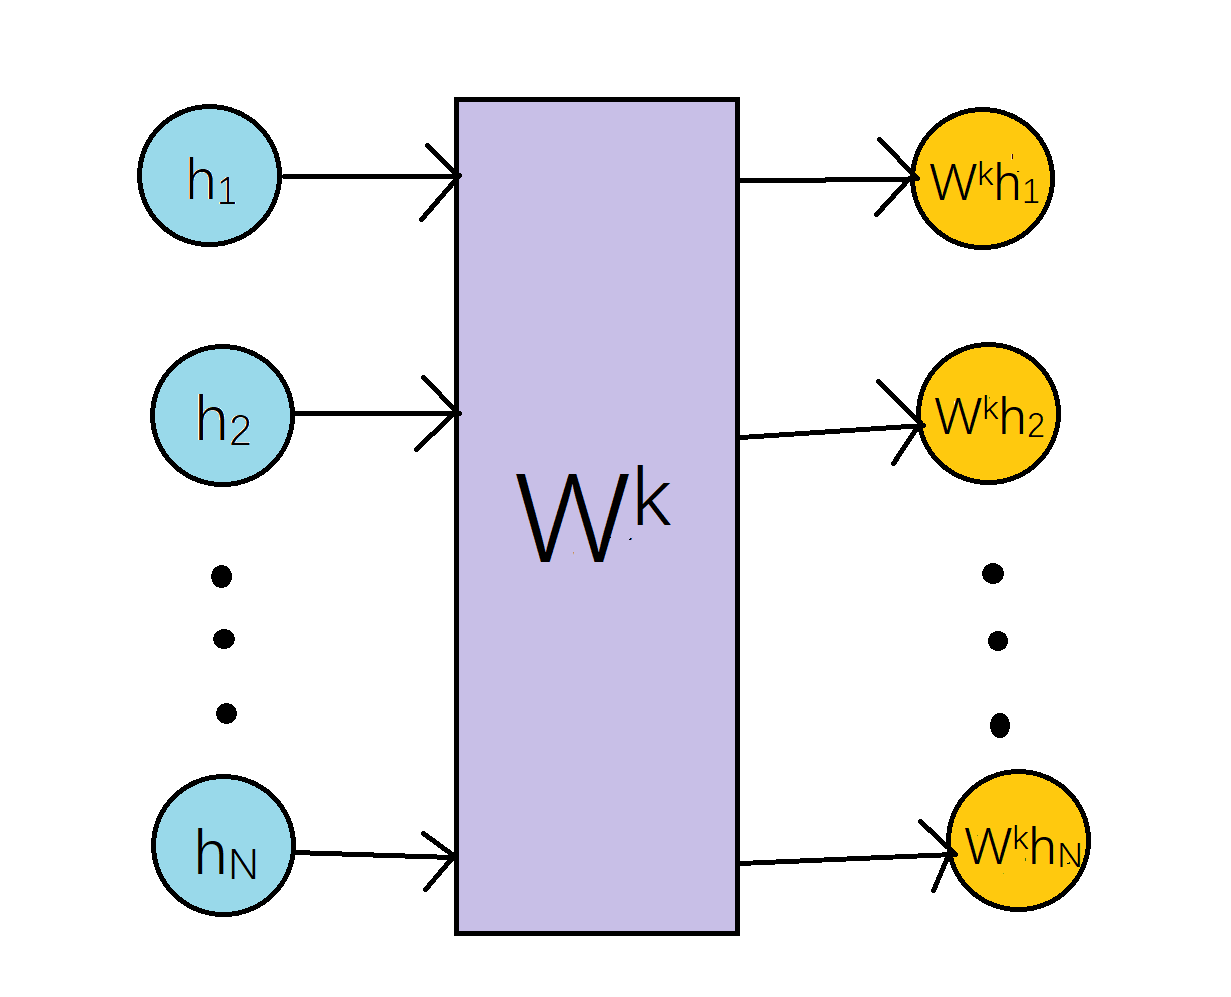
\includegraphics[width=8cm, height=4cm, scale=0.4]{images/linear.png}
\noindent\textbf{h_i\in R^{F*t}; W^k\in R^{F^{'} * F}; W^kh_i \in R^{F^{'} * t}}    
\end{frame}

\begin{frame}{attentional mechanism}
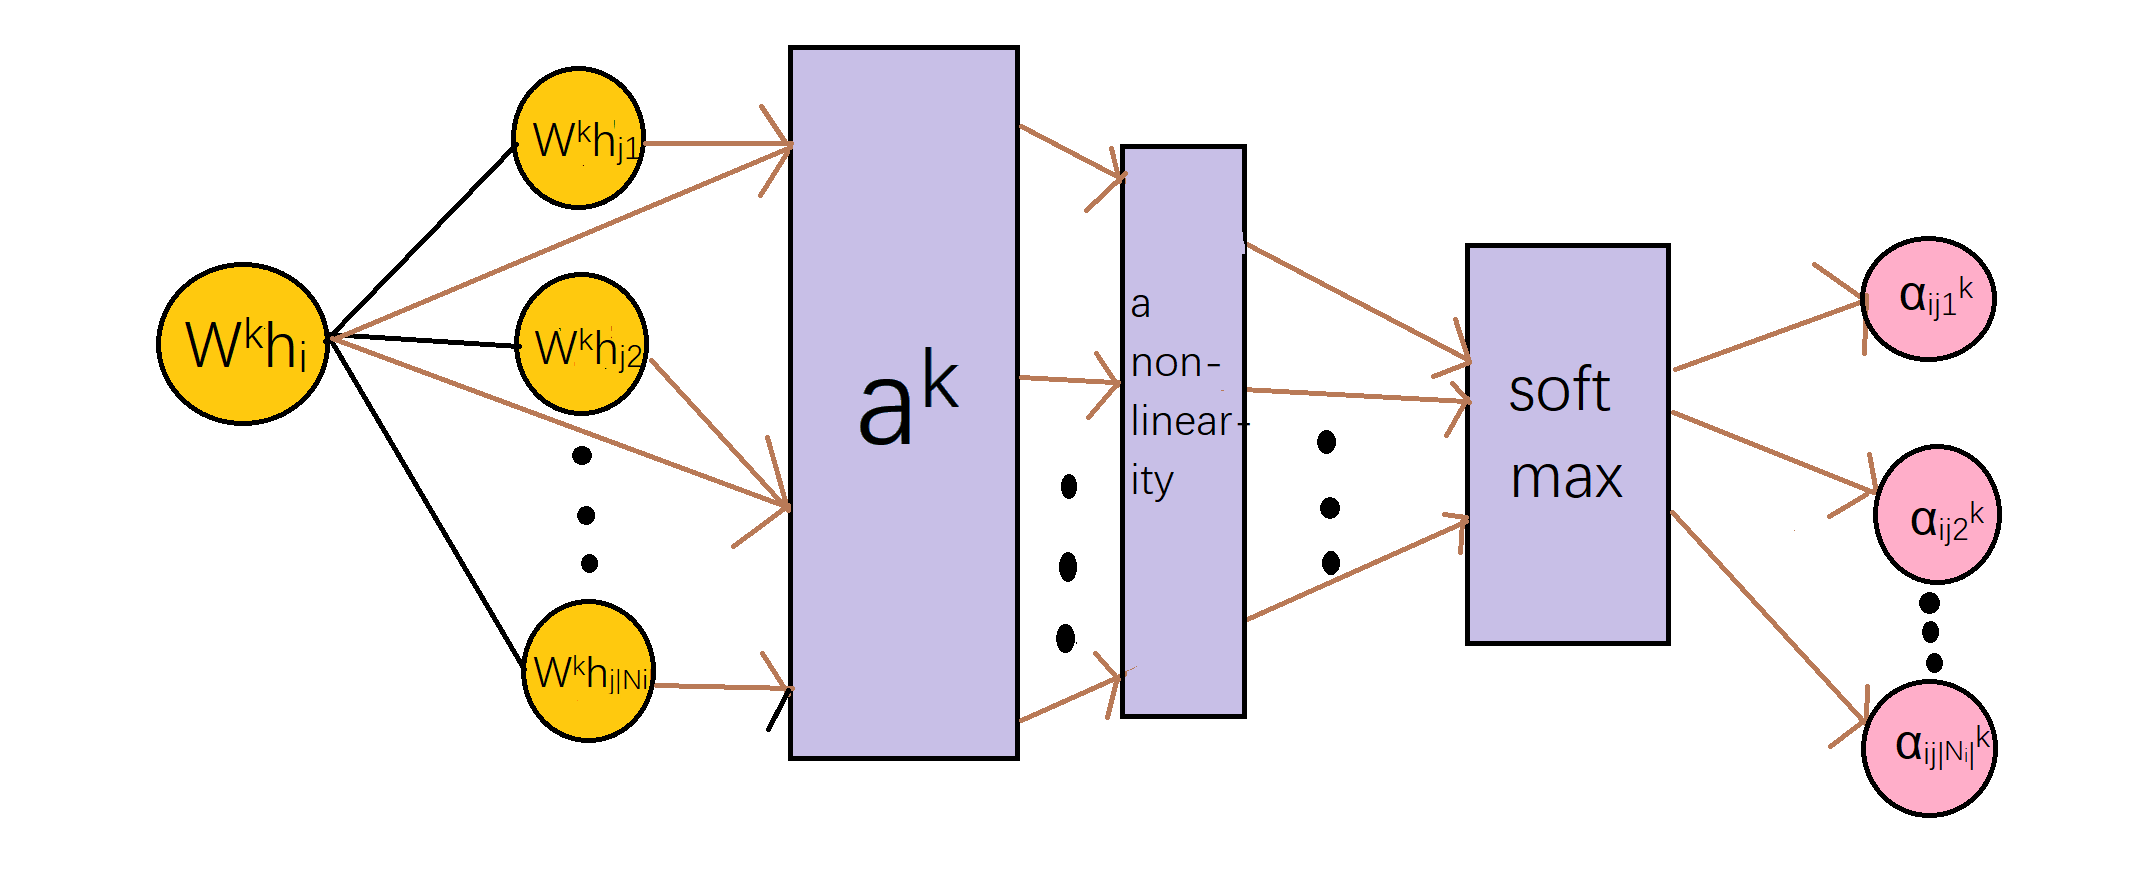
\includegraphics[width=12cm, height=6cm, scale=0.4]{images/softmax (2).png}
\noindent\textbf{W^{k}h_i \in R^{F^{'}*t}; j1, j2,...,j|N_i| \in N_i}
\noindent\textbf{N_i is neighborhood of node i(including i); a^k \in R^{2F^'}}
\end{frame}

\begin{frame}{}
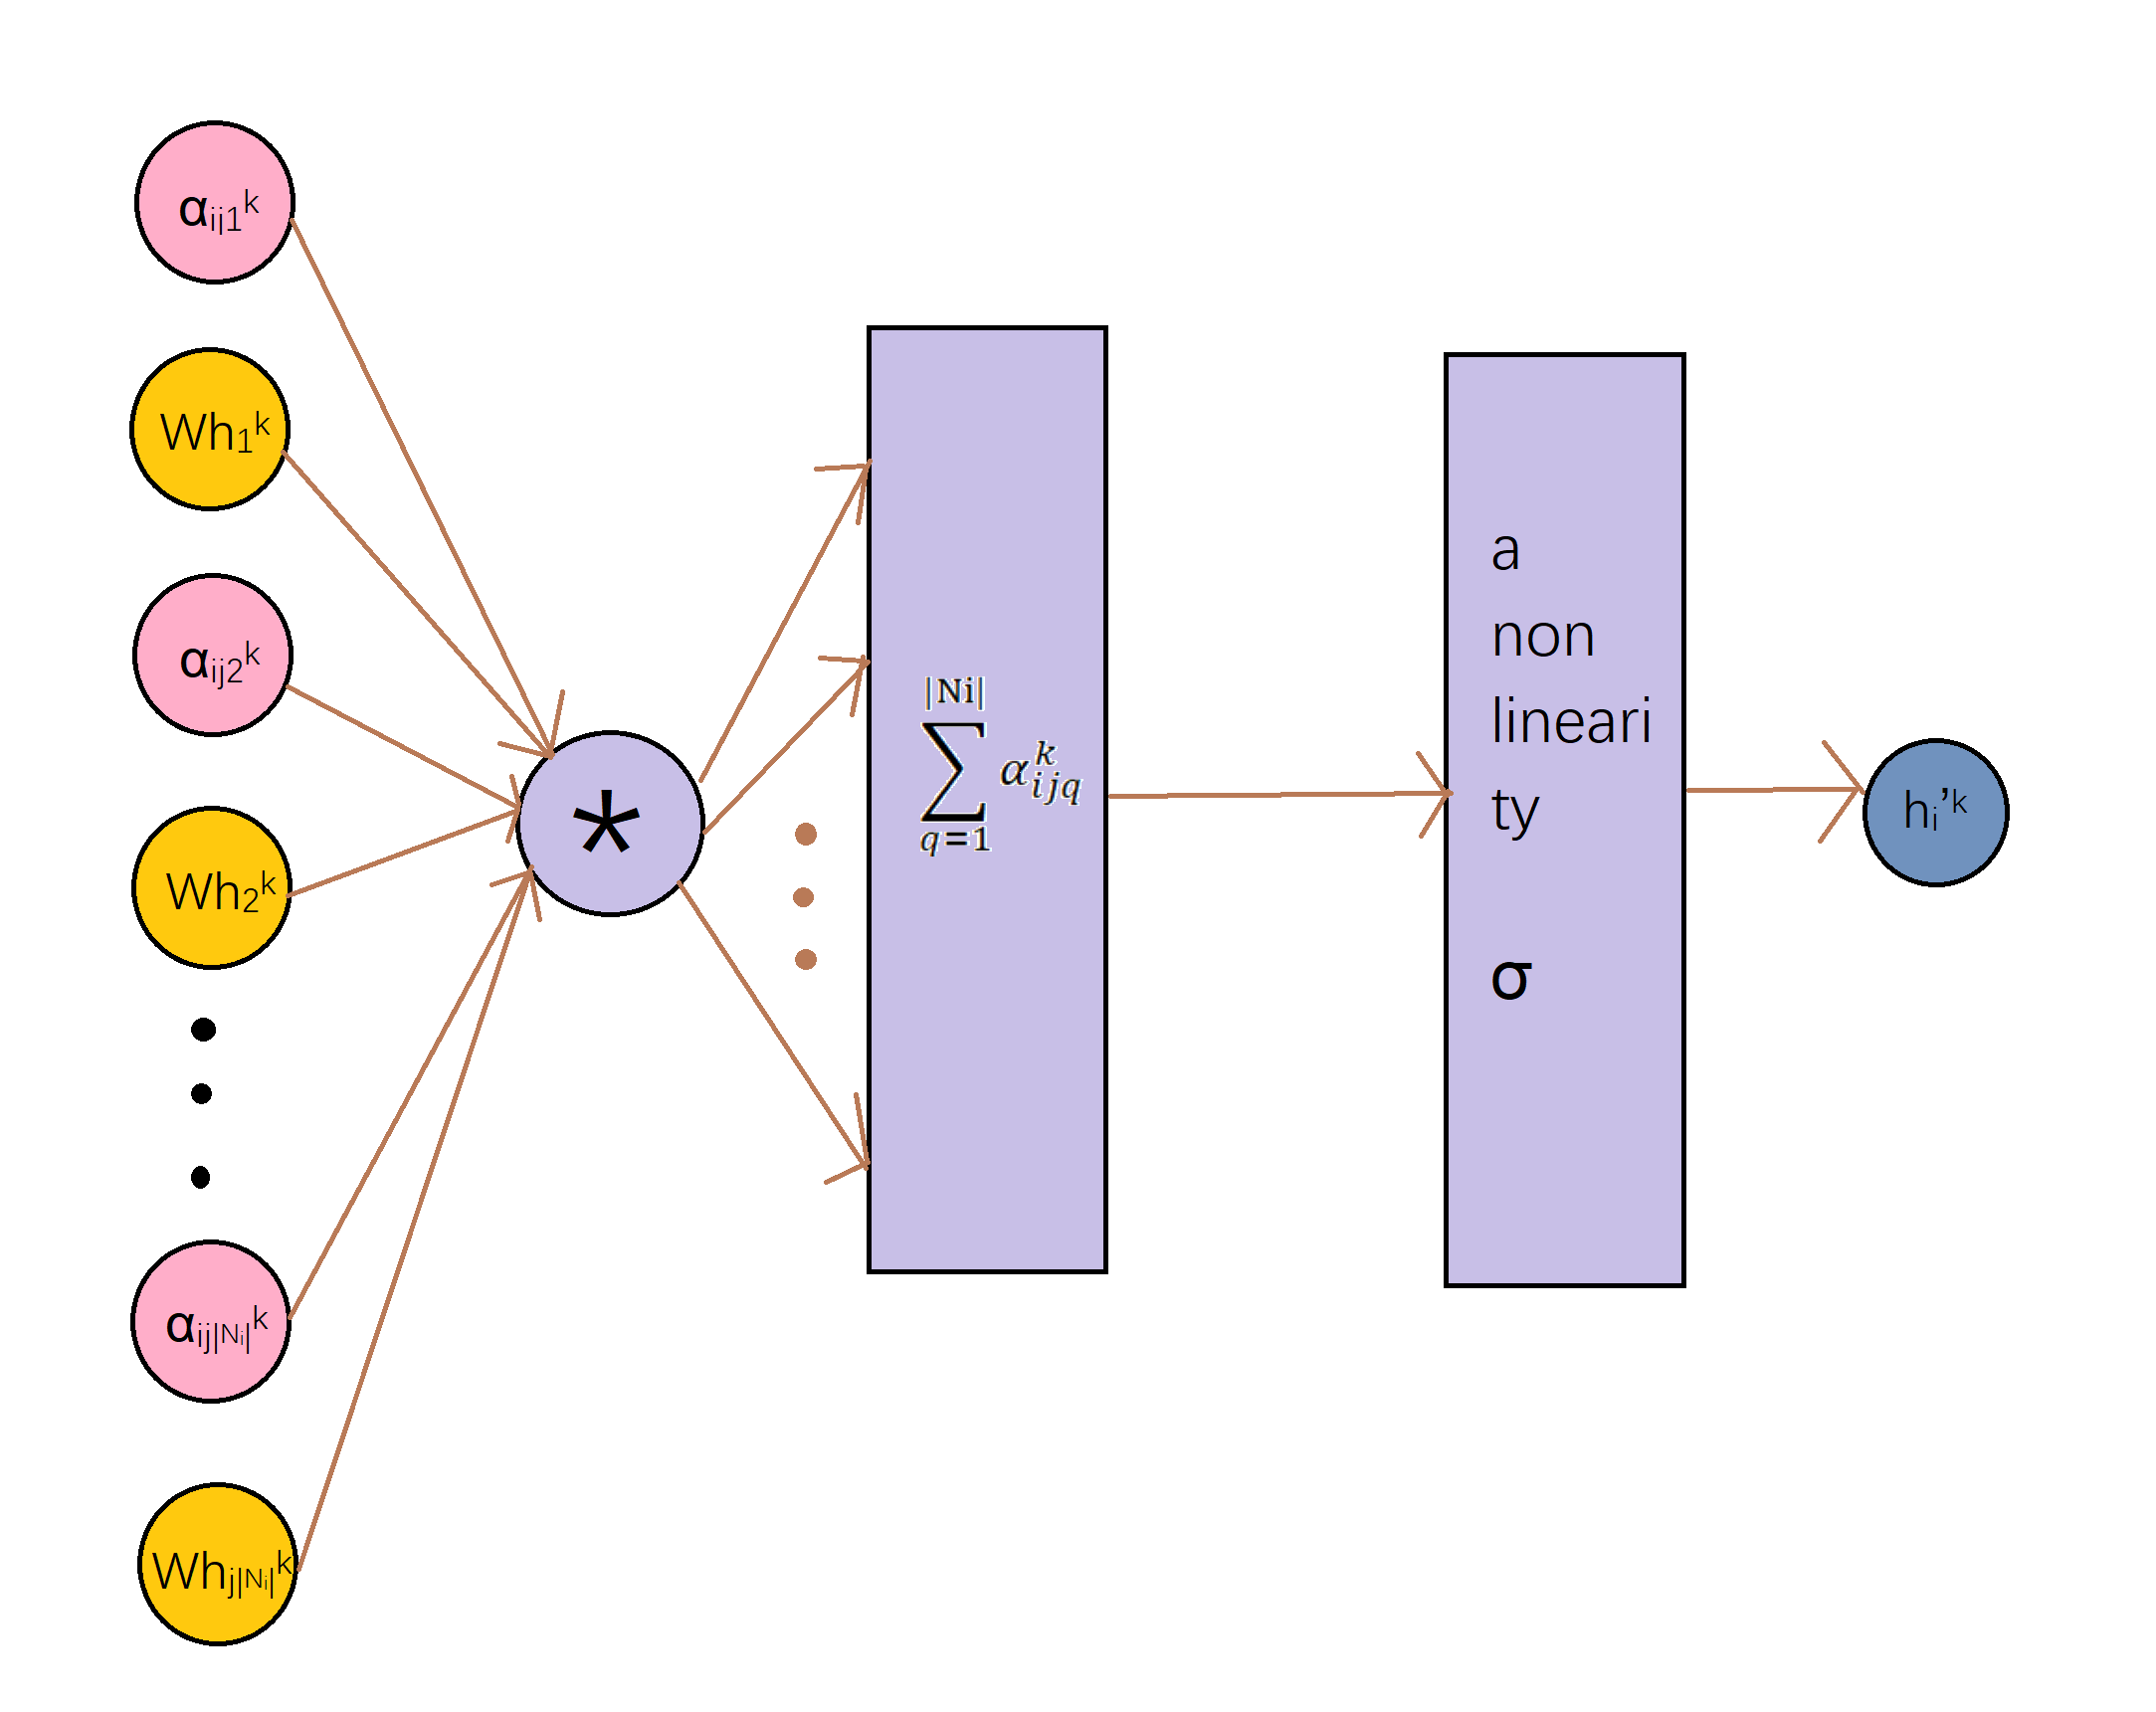
\includegraphics[width=12cm, height=6cm, scale=0.4]{images/h (2).png}
\noindent\textbf{h_i^{'k} \in R^{F^{'}*t}}
\end{frame}

\begin{frame}{}
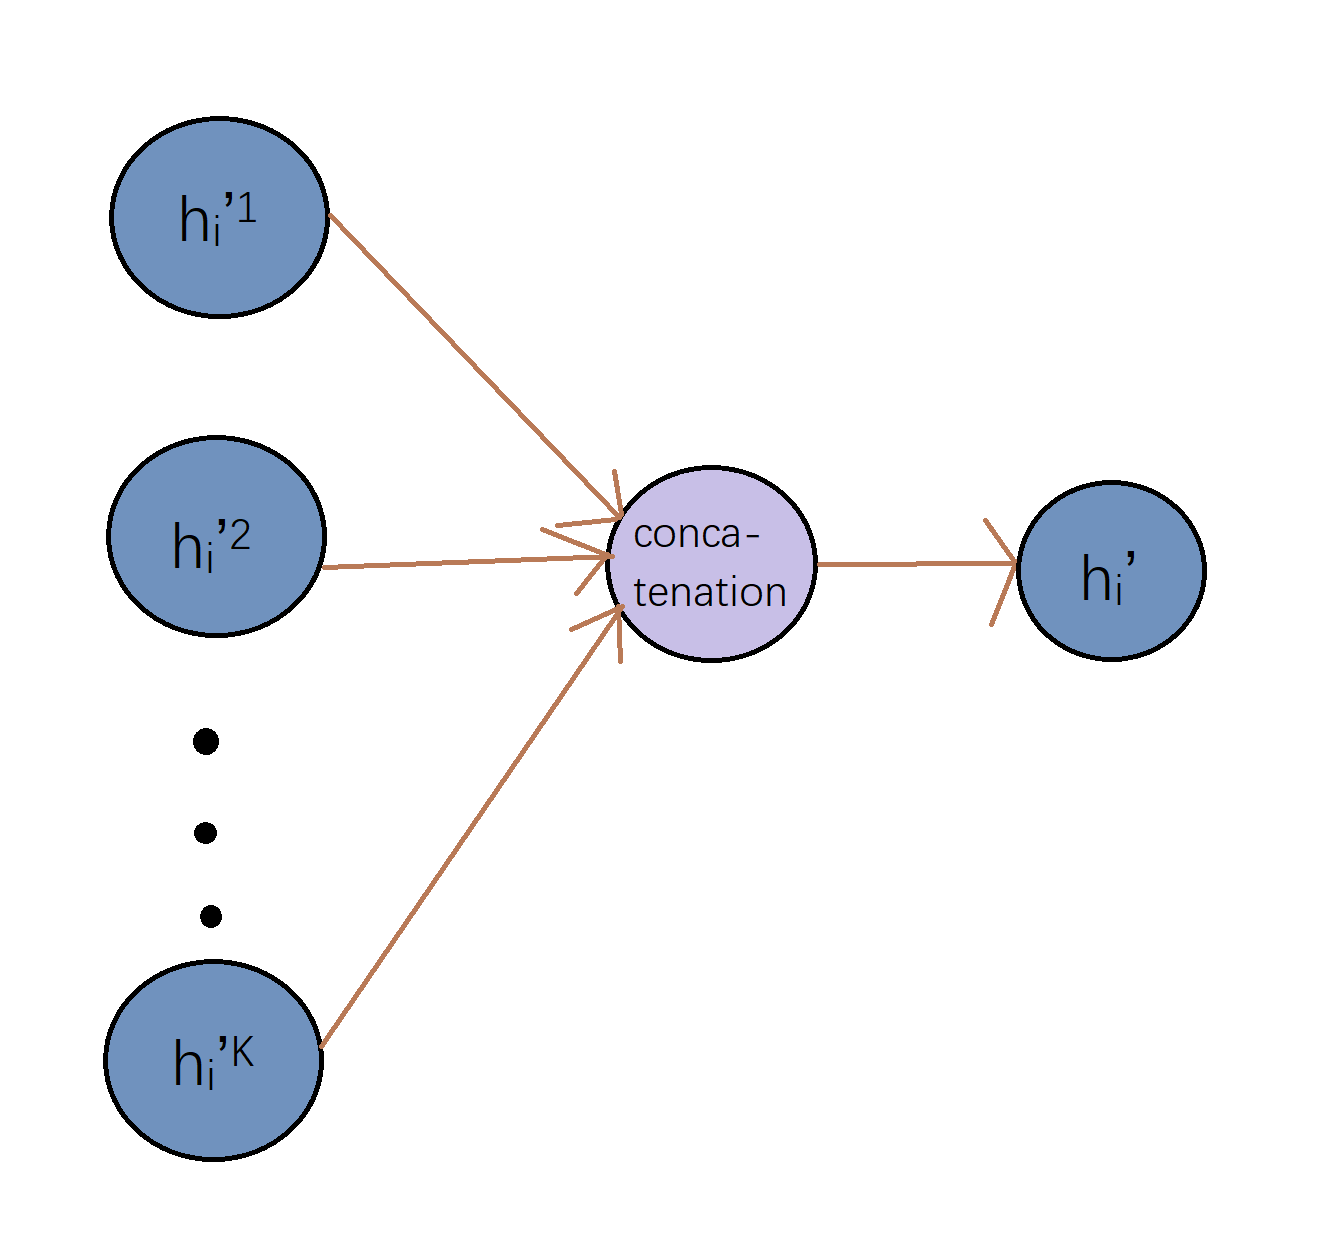
\includegraphics[width=12cm, height=6cm, scale=0.4]{images/h2 (2).png}
\noindent\textbf{h_i^' \in R^{KF^{'}*t}}
\end{frame}







% \end{document}


% \documentclass[compress,xcolor=table]{beamer}

% % Packages
% \usepackage[english]{babel}
% \usepackage[utf8]{inputenc}
% \usepackage[T1]{fontenc}
% \usepackage{datetime}

% % Possible options of the package (add/remove below in \usetheme call):
% %  - nosectionpages: no pages between sections
% %  - flama: use flama font, requires xelatex/lualatex + the font to compile
% %  - compressminiframes: put the heading list bullets indications pages on 1 line
% \usetheme[compressminiframes]{sorbonne}

% % Title page
% \title{Lorem Ipsum \newline Dolor Sit Amet}
% \foottitle{Lorem Ipsum Dolor Sit Amet} % optional, printed at the bottom of the slides, by default same as title, can be useful to rewrite when title has a newline for example
% \subtitle{Subtitle} % optional subtitle
% \date{\formatdate{22}{03}{2018}}
% \author{Prénom Nom}
% % \institute{LIP6 - Sorbonne Université} % Optional

% % Biblatex
% \usepackage[backend=bibtex, style=authoryear, citestyle=authoryear]{biblatex}
% \bibliography{library.bib}
% \renewcommand*{\bibfont}{\footnotesize}


% %%%%
% %% BEGIN OF SLIDES
% %%%%

% \begin{document}

% \begin{frame}[plain]
% 	\titlepage
% 	\setcounter{framenumber}{0}
% \end{frame}


\section{Deep Survival Analysis} \subsection{}

\begin{frame}{Survival Analysis(SA)}
	
	\begin{alertblock}{The problem}
		
		\begin{itemize}
			\item To analyze the expected duration of time until one or more events happen.
% 			\item
% 			It contains a certain amount of noise
		\end{itemize}
		
	\end{alertblock}
	
	\begin{block}{Task of SA}
		
		\begin{itemize}
			\item
			the probability of event happening at each time: $p(z)$
			\item
		     the probability of event happened at that time: $W(t)$
			\item
			the probability of event not happened at the time: $S(t)$
		\end{itemize}
		
	\end{block}
	
\end{frame}

\begin{frame}{Challenges in SA}
	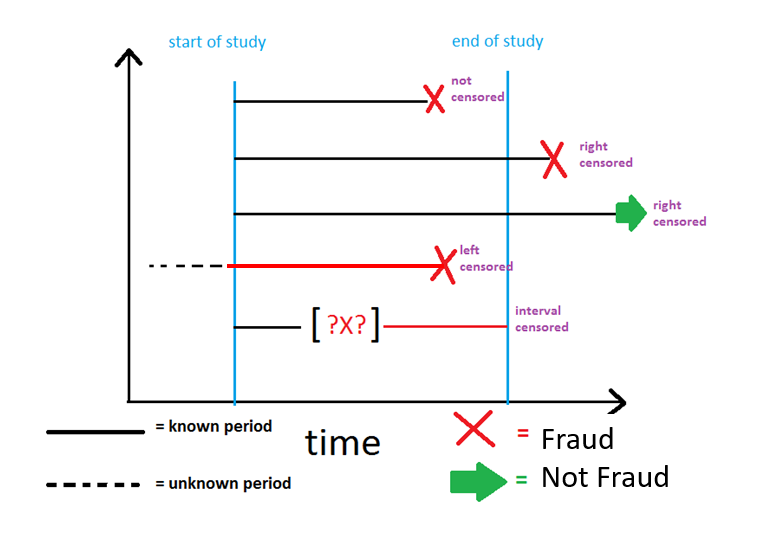
\includegraphics[width=12cm, height=6cm, scale=0.4]{images/01.png}

	
\end{frame}

\begin{frame}{Existing Methods}
	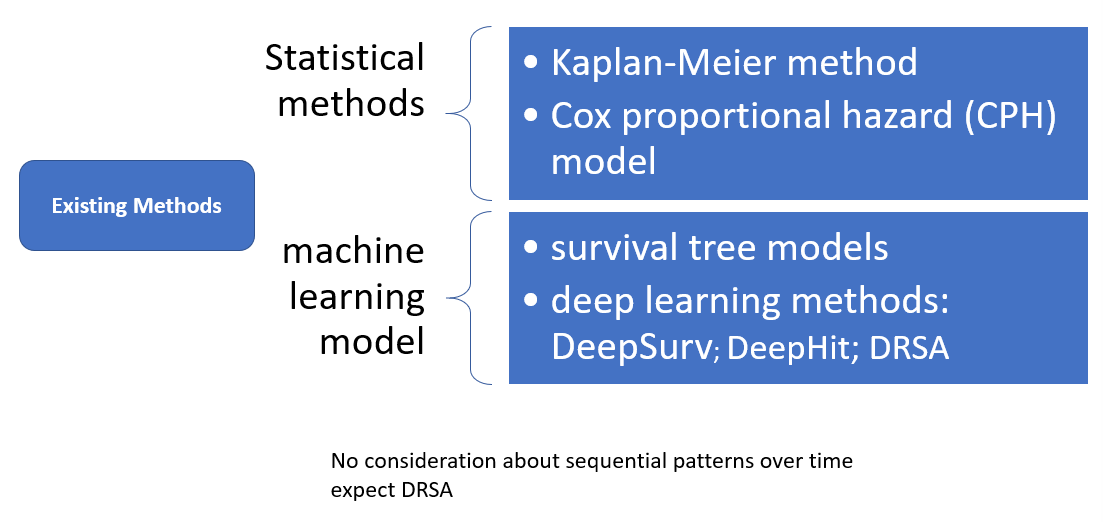
\includegraphics[width=11cm, height=6cm, scale=0.4]{images/02.png}

	
\end{frame}

\begin{frame}{Deep Recurrent Survival Analysis (DRSA)[6]}

	\begin{block}{Pros}
		\begin{itemize}
			\item No assumption about distributional forms
			\item Captures sequential patterns in the feature-time space
			\item First work ever, utilizes auto-regressive model for SA
			\item Handling censorship with unbiased learning
			\item Significant improvement against both stat. methods and ML methods
		\end{itemize}
		
	\end{block}
	
\end{frame}

\begin{frame}{Model diagram}
	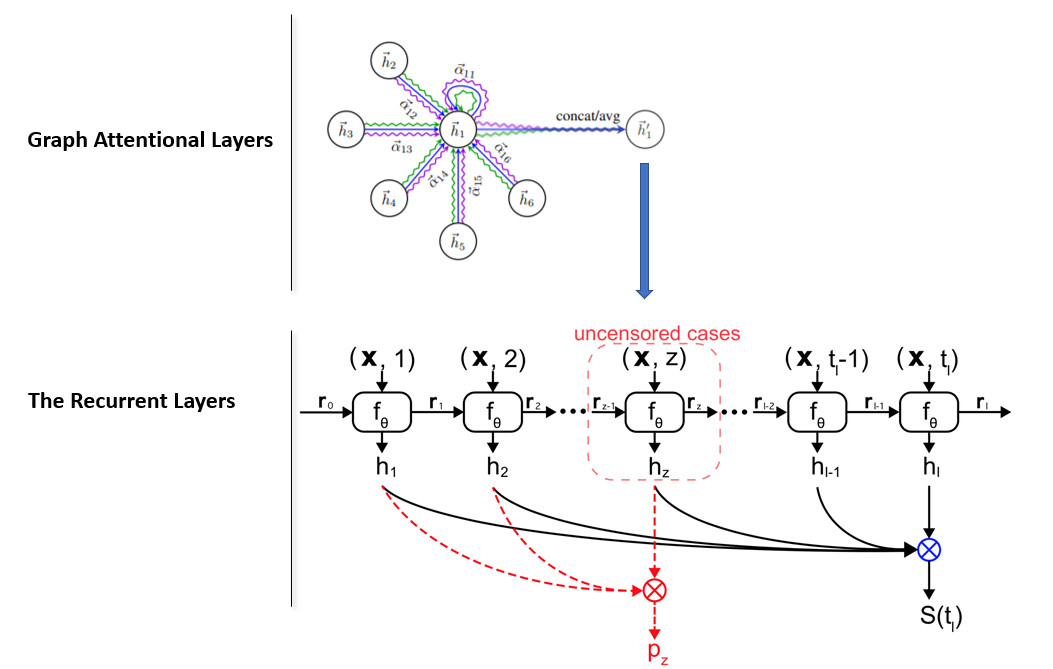
\includegraphics[width=12cm, height=6cm, scale=0.4]{images/03.png}

	
\end{frame}

% \section{References} \subsection{}

% \begin{frame}[allowframebreaks]{References}
	
% 	\printbibliography[heading=none]
	
% \end{frame}




% \end{document}


\begin{frame}{References}
	
\begin{thebibliography}{99}
\bibitem{1}Kim M J,Kim T S A neural classifier with fraud density map foreffective credit card fraud detection[C]
\bibitem{2}《基于CNN的信用卡欺诈检测》
\bibitem{3}《Unsupervised profiling methods for fraud detection》
\bibitem{4}《Analysis of credit card fraud detection methods》[J]
\bibitem{5} 《基于图特征的欺诈检测方法研究与应用》
\bibitem{6} Ren, Kan et al. (2019). Deep Recurrent Survival Analysis
\end{thebibliography}
	
\end{frame}




\end{document}

